\section{Exploration and Analysis}
    \subsection{What makes a movie successful?}
        % We would like you to explore what makes a movie popular and/or successful.
        \paragraph{}
            In order to ascertain which factors are most influential in determining the
                success of a movie, it is necessary to first define what constitutes success.
            For the purpose of this analysis, success is defined as the movie's revenue.
            By examining the correlations between the movie's revenue and other factors, we
                can gain insight into which factors have the greatest impact on the success of
                a movie.
            These correlations are visualised in Figure \ref{fig-heatmap}.

            \begin{figure}[H]
                \centering
                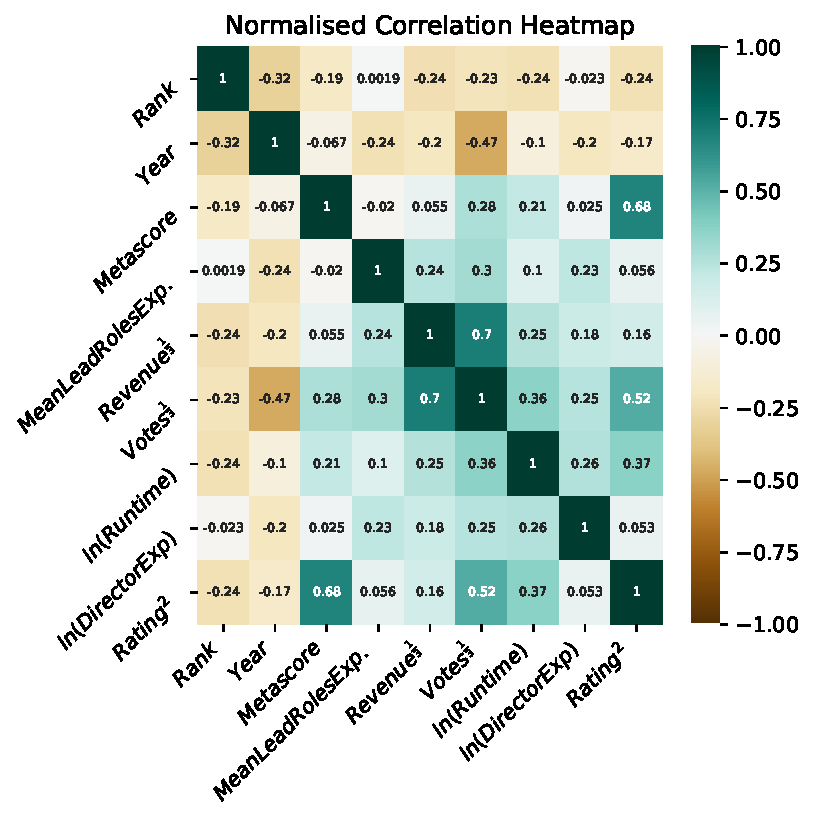
\includegraphics[width=0.8\linewidth]{Final/Normalised Correlation Heatmap.pdf}
                \caption[short]{
                    A heatmap illustrating the strength of correlations between various normalised
                    variables from the IMDb dataset \cite{data:IMDb}.
                    The Pearson's Product Moment Correlation Coefficient is used to calculate the
                        strength of the correlations.
                    These variables included Rank, Year, Metascore, Revenue, Votes, Runtime, and
                        Rating.
                    Additionally, two more variables were calculated from the TMD data
                        \cite{data:TMD}: MeanLeadRolesExperience and DirectorExperience.
                    Each correlation is represented by a value between -1 and 1, with weaker
                        correlations having values closer to 0, and negative correlations having
                        negative values and positive correlations having positive values.
                }\label{fig-heatmap}
            \end{figure}

        \paragraph{}
            Figure \ref{fig-heatmap} reveals a strong positive correlation (0.7) between a
                movie's revenue and the number of votes it receives on IMDb, suggesting that
                the more votes a movie receives, the higher its revenue is likely to be.
            Additionally, the heatmap shows moderate positive correlations between the
                movie's revenue and its runtime (0.25) and between the movie's revenue and the
                experience of the actors in lead roles (0.24), indicating that longer runtimes
                and more experienced actors may be associated with higher revenues.
            In contrast, there is a moderate negative correlation between a movie's revenue
                and its rank on IMDb (-0.24), suggesting that higher ranks on IMDb do not
                necessarily translate to higher revenues.
            These four correlations are shown in more detail in Figure
                \ref{fig-revenue-factors}.

            \begin{figure}[H]
                \centering
                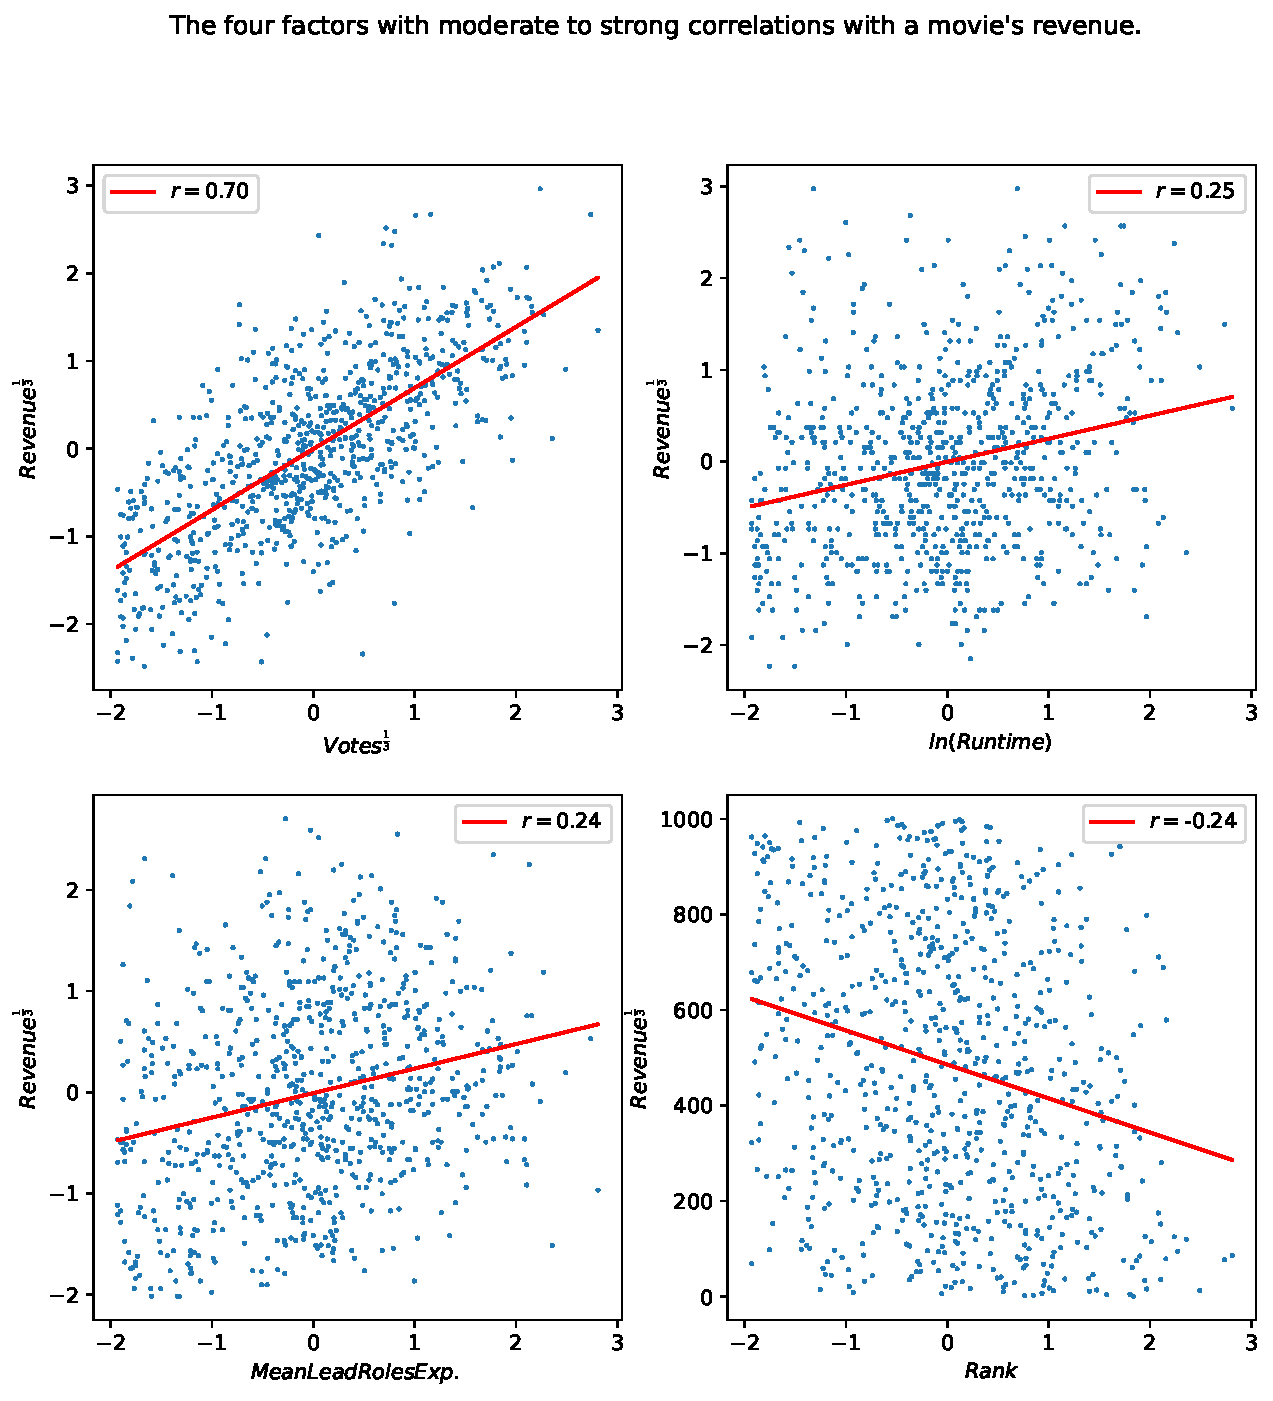
\includegraphics[width=0.8\linewidth]{Final/Revenue Factors.pdf}
                \caption[short]{
                    Scatter plots showing the relationships between a movie's revenue and the four
                    factors with moderate or strong correlations.
                }\label{fig-revenue-factors}
            \end{figure}

    \subsection{The relationship between a movie's ranked position and its number of votes}
        % We would also like you to visualise the distribution of ranked position and
        % number of votes, and comment on the relationship between them.
        \paragraph{}
